% ===========================================================================
%  SECTION-STYLE APPENDIX -- for structure = sections only.
%  The chapters-mode counterpart is chapters/chapter-style-appendix.tex.
%
%  An appendix is written like any other top-level division, so in this mode
%  its title is a \section and its subheadings are \subsection. It still
%  prints the way every other major division does -- centred and uppercase at
%  the top of a fresh page. \ThesisAppendices in main.tex counts the appendix
%  files listed there: two or more get "APPENDIX A", "APPENDIX B" above their
%  titles and figures and tables numbered A.1, B.1, while a lone appendix gets
%  a bare "APPENDIX" and figures and tables numbered 1, 2.
%
%  The line below stops the build if this file is used in a chapters document,
%  where \section would quietly turn it into a subheading of the appendix
%  before it. Use chapter-style-appendix.tex there instead.
% ===========================================================================
\ThesisSectionsOnly

\section{Supplementary Material}

Supporting material that would interrupt the argument belongs here rather than
in the body: extended derivations, full instrument settings, code listings,
questionnaire text, or the signed AI Use Agreement if one is required.

Each appendix is a separate file with its own \verb|\chapter| command and its
own \verb|\input| line in \verb|main.tex|, exactly like a chapter. The
\verb|\ThesisAppendices| line above those inputs is all the setup there is:
two or more appendix files are lettered A, B, C, with their tables and figures
numbered A.1, B.1 and so on, while a single appendix file prints an unlettered
``APPENDIX'' and numbers its tables and figures 1, 2, 3.

\subsection{An Appendix Subheading}

Appendix subheadings are styled like the ones in the body but are left out of
the table of contents, which lists appendix titles only. Tables and figures
inside an appendix carry the appendix letter, where there is one, and are
listed in the List of Tables and the List of Figures either way.

\begin{table}
  \caption{Instrument settings used throughout the study.}
  \label{tab:sec-appendix-settings}
  \begin{tabular}{lr}
    \toprule
    Setting & Value \\
    \midrule
    Sampling rate (Hz) & 1000 \\
    Gain               &   10 \\
    \bottomrule
  \end{tabular}
\end{table}

\begin{figure}
  \centering
  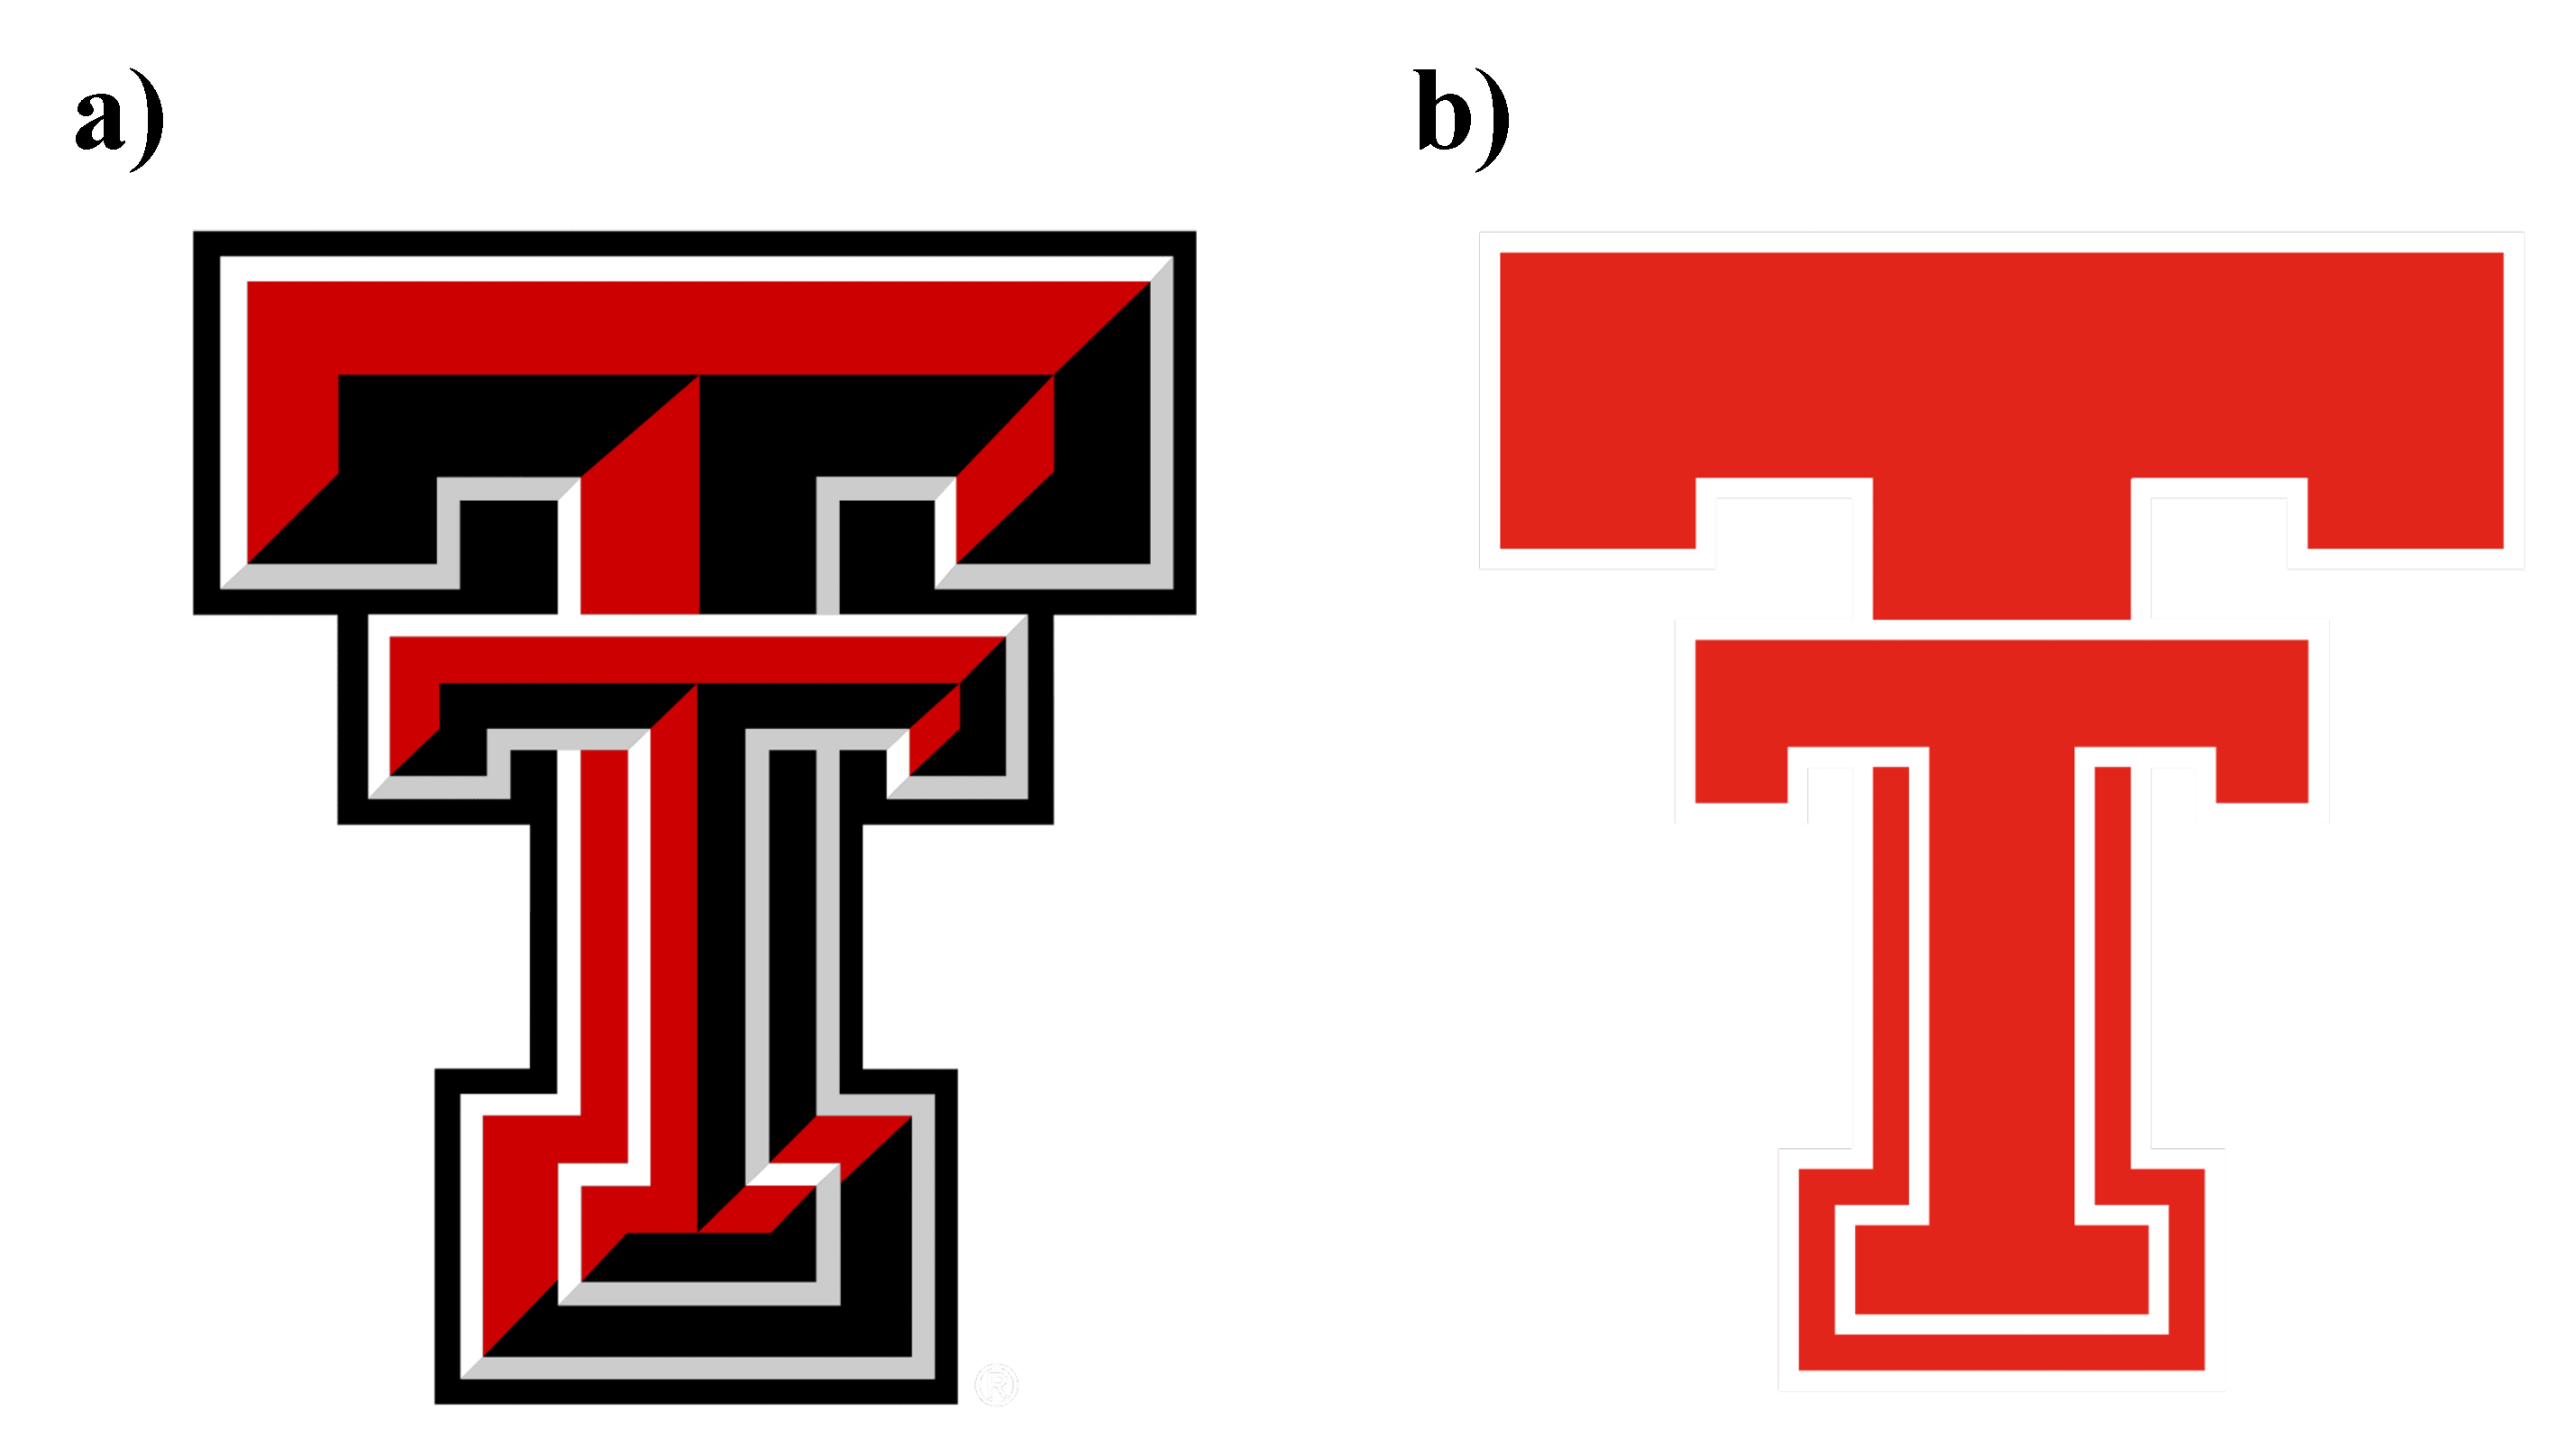
\includegraphics[height=2.2in,
    alt={A supplementary comparison of the retro and current Texas Tech University Double-T
    logos}]{figures/example-Double-T.pdf}
  \caption{Demonstrating multiple appendecies with the Double T logos.}
  \label{fig:doublet2}
\end{figure}
